\ifx\wholebook\relax \else

\documentclass[b5paper]{ctexart}
\usepackage[nomarginpar
  %, margin=.5in
]{geometry}

\addtolength{\oddsidemargin}{-0.05in}
\addtolength{\evensidemargin}{-0.05in}
\addtolength{\textwidth}{0.1in}
\usepackage[cn]{../../../prelude}

\setcounter{page}{1}

\begin{document}

\title{二叉堆}

\author{刘新宇
\thanks{{\bfseries 刘新宇 } \newline
  Email: liuxinyu95@gmail.com \newline}
  }

\maketitle
\fi

\markboth{二叉堆}{基本算法}

\ifx\wholebook\relax
\chapter{二叉堆}
\numberwithin{Exercise}{chapter}
\fi

\section{定义}
\label{introduction} \index{二叉堆}

堆是一种常见的数据结构,可以解决很多实际问题,包括排序、带有优先级的调度、实现图算法等\cite{wiki-heap}。堆有多种实现,最常见的一种通过数组来表示二叉树\cite{CLRS},进而实现堆。许多程序库中的堆都是这样实现堆的。由R.W. Floyd给出的高效堆排序算法也利用了这个实现\cite{wiki-heapsort}\cite{rosetta-heapsort}。堆本身的定义是抽象的,除数组外,它也可以由其它数据结构来实现。本章中,我们介绍那些由二叉树实现的堆,包括左偏堆(Leftist heap)、斜堆(Skew heap)、伸展堆(splay heap)\cite{okasaki-book}。一个堆或为空,或存有若干可比较大小的元素。它满足一条性质并定义了三种操作:

\begin{enumerate}
\item \textbf{性质}:堆顶总保存着最小(或最大)元素;
\item \textbf{弹出操作}移除堆顶元素,并保持堆的性质:新的堆顶元素仍是剩余中最小(或最大)的;
\item \textbf{插入操作}将新元素加入堆中,并保持堆的性质;
\item \textbf{其它操作}(如合并两个堆)也保持堆的性质。
\end{enumerate}

我们称顶部保存最小元素的堆为\textbf{小顶堆},顶部保存最大元素的堆为\textbf{大顶堆}。可以用树来实现堆。将最小(或最大)元素置于根节点。获取“堆顶”元素时,可以直接返回根节点中的数据。执行“弹出”操作时,将根节点删除,然后从子节点重新构建树。我们称使用二叉树实现的堆为\textbf{二叉堆}。本章介绍三种不同的二叉堆。

\section{由数组实现的隐式二叉堆}
\label{ibheap} \index{隐式二叉堆} \index{完全二叉树}

第一种实现称为“隐式二叉树”。它用数组来表示一棵完全二叉树。所谓完全二叉树,是一种“几乎”满的二叉树。深度为$k$的满二叉树含有$2^k-1$个节点。如果将每个节点从上到下,从左向右编号为1,2, ..., $2^k - 1$,则完全二叉树中编号为$i$的节点和满二叉树中编号为$i$的节点在树中的位置相同。完全二叉树的叶子节点仅出现在最下面一行和倒数第二行。图\ref{fig:tree-array-map}给出了一棵完全二叉树和相应的数组表示形式。由于二叉树是完全的,对数组中第$i$个元素代表的节点,它的父节点定位到第$\lfloor i/2 \rfloor$个元素;左子树对应第$2i$个元素,而右子树对应第$2i+1$个元素。如果子节点的索引超出了数组的长度,说明它不含有相应的子树(例如叶子节点)。树和数组之间的映射可以定义如下(令数组的索引从1开始):

\begin{figure}[htbp]
\centering
   \includegraphics[scale=0.45]{img/tree-array-map-tree}
   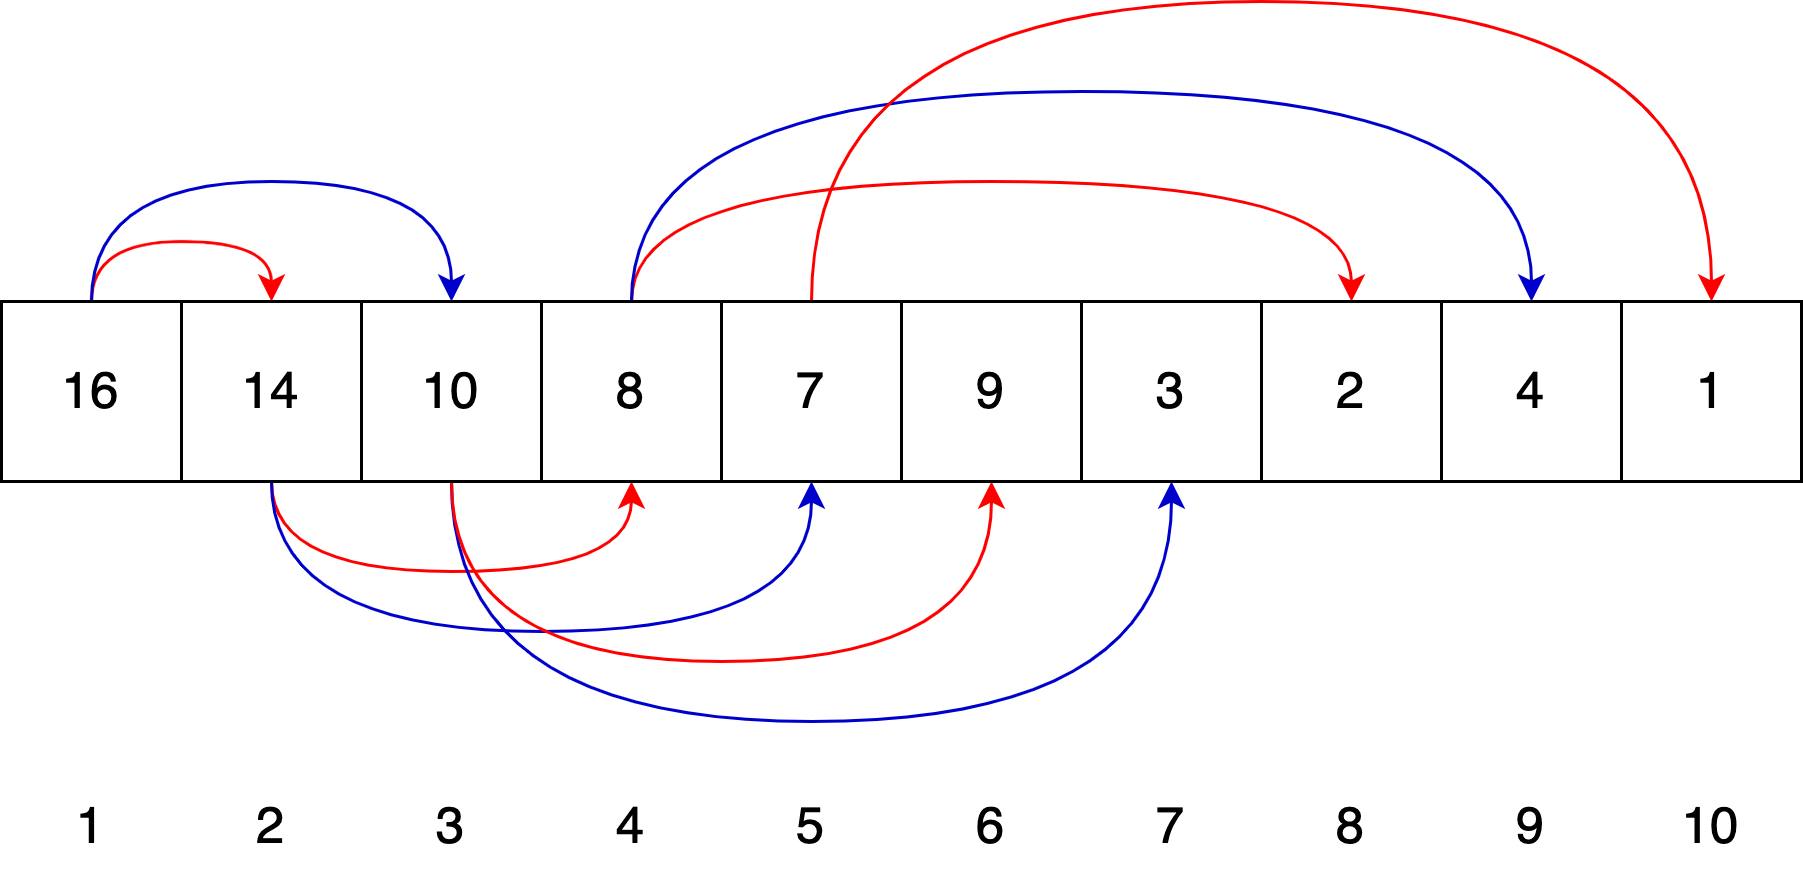
\includegraphics[scale=0.5]{img/binary-tree-in-array}
 \caption{完全二叉树到数组的映射} \label{fig:tree-array-map}
\end{figure}

\be
\begin{cases}
parent(i) & = \lfloor \dfrac{i}{2} \rfloor \\
left(i)   & = 2i \\
right(i)  & = 2i + 1 \\
\end{cases}
\ee

父节点和子树的访问可以通过位运算实现,见本章附录中的例子。

\subsection{堆调整}
\index{二叉堆!Heapify}

堆调整\footnote{Heapify,也译作堆化。}是维护堆性质的过程,使得堆顶元素为最小(或最大)。由于堆背后的数据模型是二叉树,我们可以利用树的递归特性,获得一个增强的堆性质:使得每棵子树的根节点都是最小(或最大)的。也就是说任何子树都代表一个子堆。简单起见,我们考虑小顶堆。对于用数组表示的二叉堆,任给数组下标$i$,我们检查$i$对应的所有子节点的值是否都不小于($\geq$)它。如果不满足则交换,使得父节点总保存最小值\cite{CLRS},并对以$i$为根的所有子树递归重复这个过程。如下算法定义了堆调整过程:

\begin{algorithmic}[1]
\Function{Heapify}{$A, i$}
  \State $n \gets |A|$
  \Loop
    \State $s \gets i$ \Comment{$s$指向最小}
    \State $l \gets$ \Call{Left}{$i$}, $r \gets$ \Call{Right}{$i$}
    \If{$l \leq n$ 且 $A[l] < A[i]$}
      \State $s \gets l$
    \EndIf
    \If{$r \leq n$ 且 $A[r] < A[s]$}
      \State $s \gets r$
    \EndIf
    \If{$s \neq i$}
      \State \textproc{Exchange} $A[i] \leftrightarrow A[s]$
      \State $i \gets s$
    \Else
      \State \Return
    \EndIf
  \EndLoop
\EndFunction
\end{algorithmic}

对于数组$A$和索引$i$,堆性质要求$A[i]$的子节点都不应比它小。否则,我选出最小的元素保存在$A[i]$,并将较大的元素交换至子树,然后自顶向下检查并调整堆,使得所有子树都满足堆性质。\textproc{Heapify}的时间复杂度为$O(\lg n)$,其中$n$是元素个数。这是因为算法中的循环次数和完全二叉树的高度成正比。图\ref{fig:heapify}描述了\textproc{Heapify}从索引2开始,按照小顶堆调整数组[1, 13, 7, 3, 10, 12, 14, 15, 9, 16]的步骤。数组最终变换为[1, 3, 7,9, 10, 12, 14, 15, 13, 16]。

\begin{figure}[htbp]
  \centering
  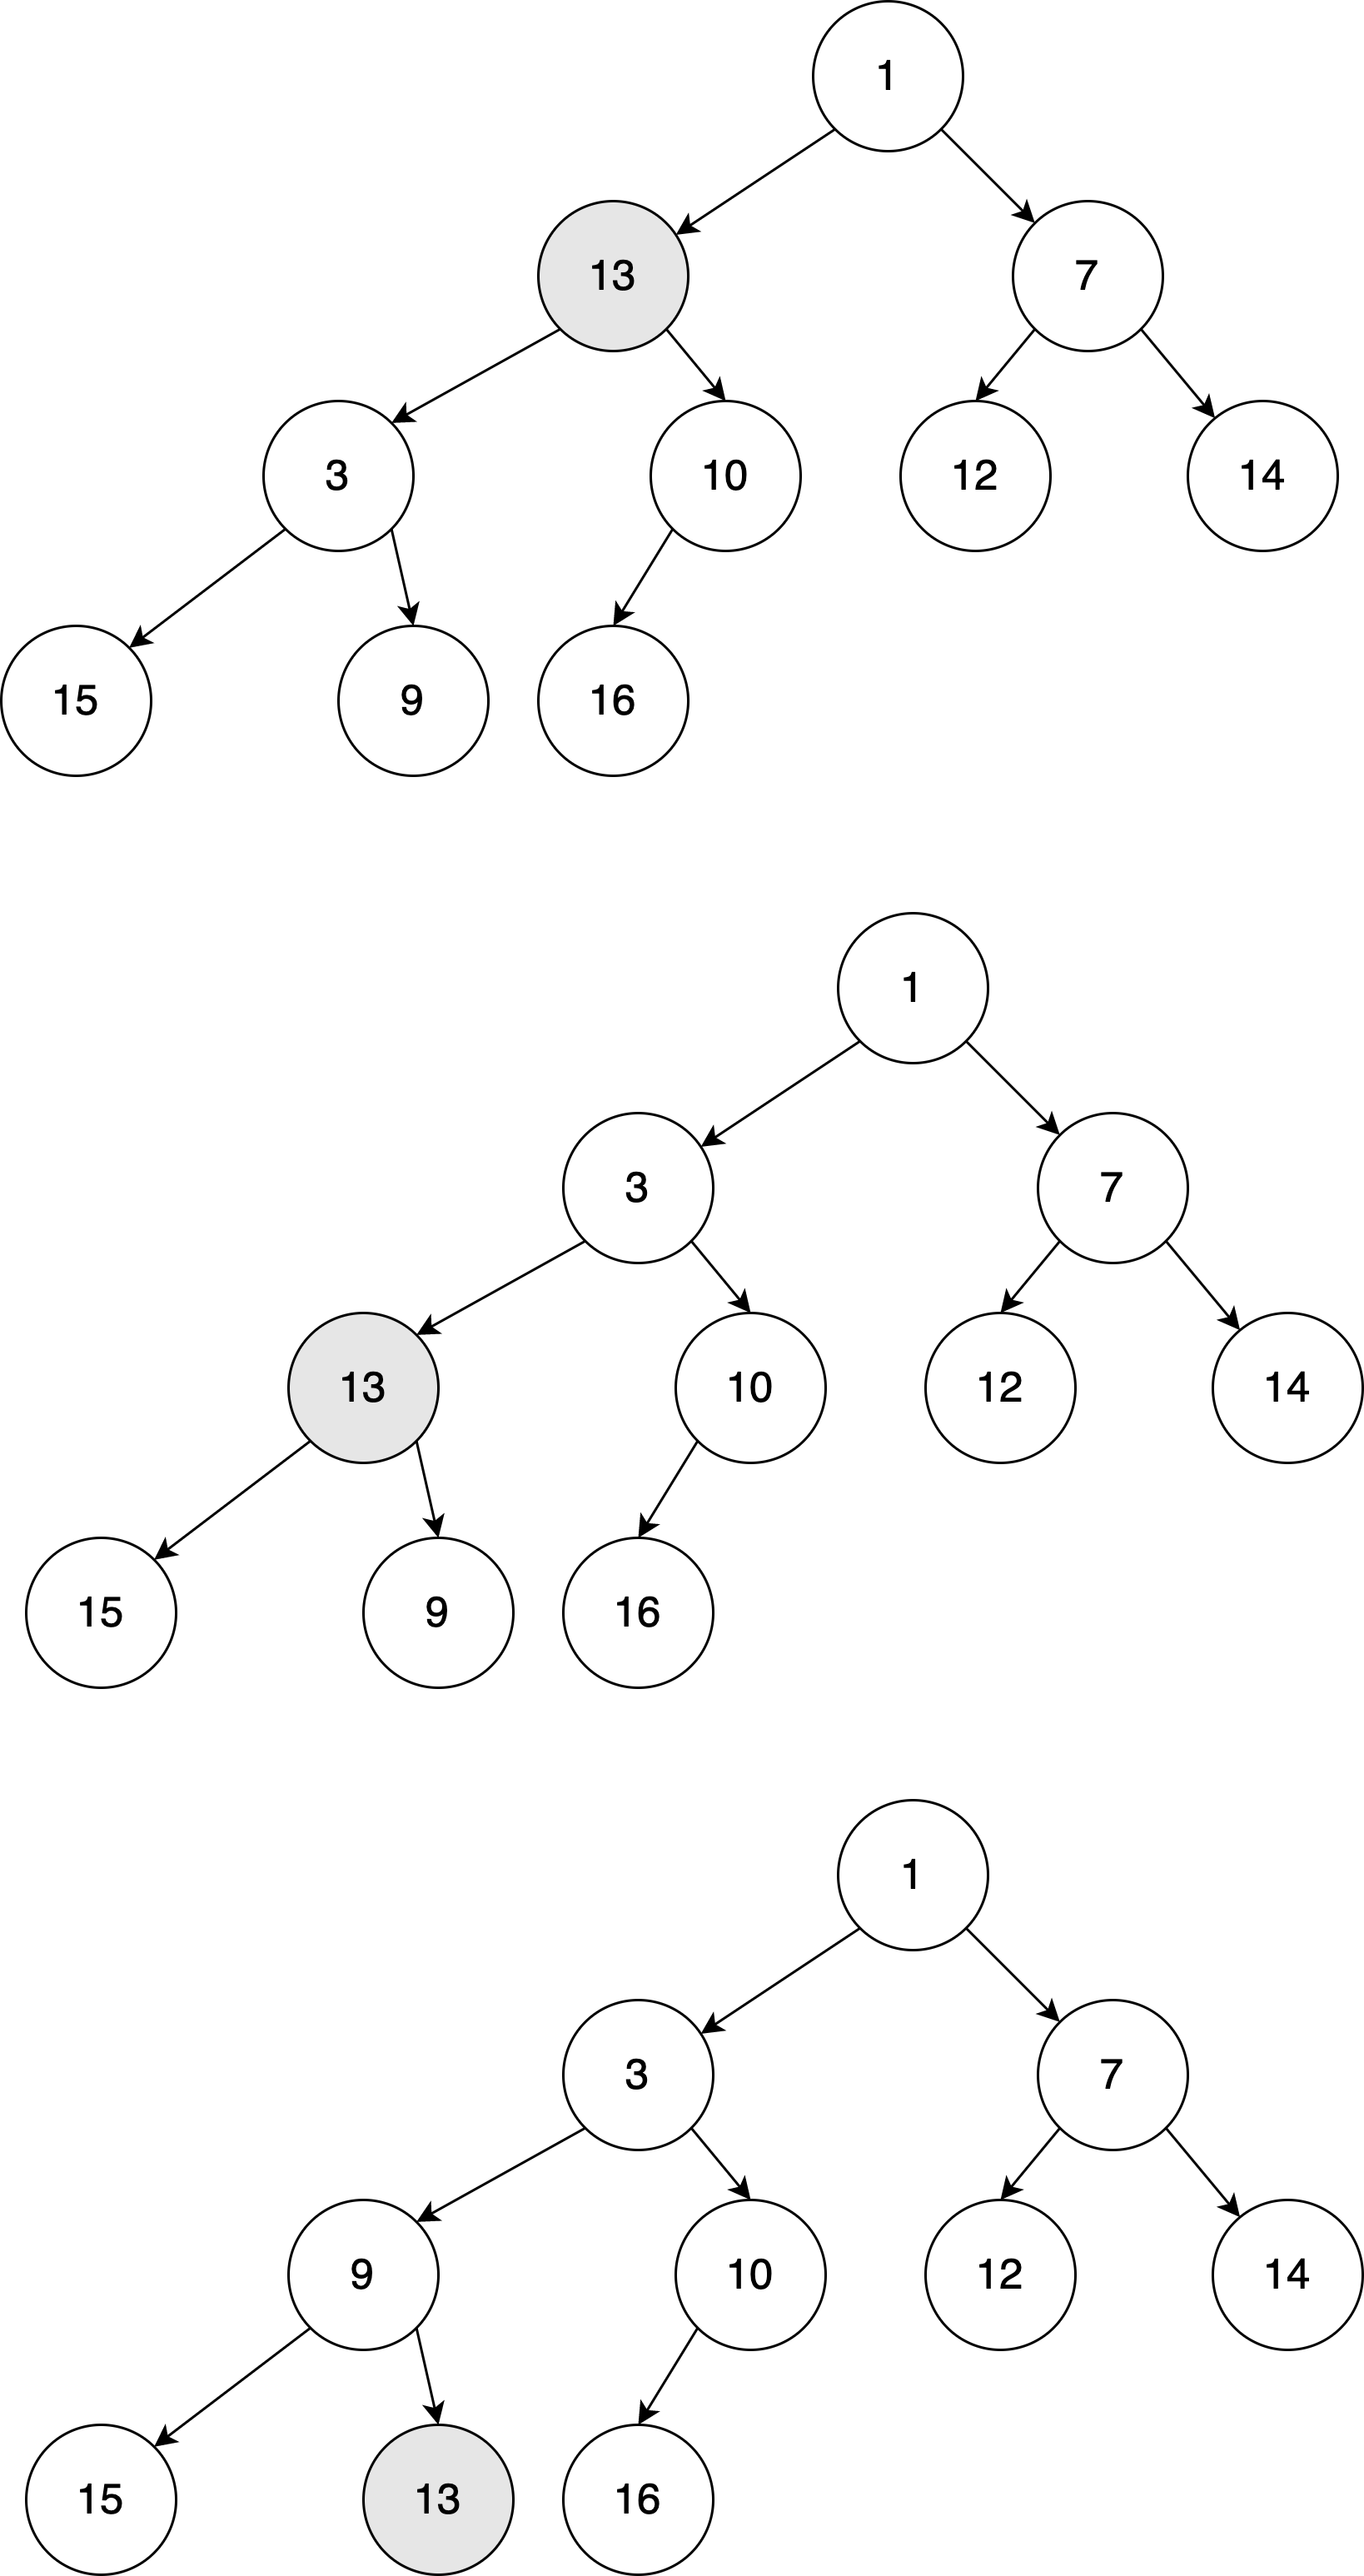
\includegraphics[scale=0.5]{img/heapify}
  \caption{堆调整。第一步:13、3、10中最小值为3,交换3 $\leftrightarrow$ 13;第二步:13、15、9中最小值为9,交换13 $\leftrightarrow$ 9;第三步:13为叶子节点,调整结束。}
  \label{fig:heapify}
\end{figure}

\subsection{构造堆}
\index{二叉堆!构造堆}

使用\textproc{Heapify},我们可以从任意数组构造出堆。观察完全二叉树各层的节点数目:$1, 2, 4, 8, ...$都是2的整数次幂,唯一例外是最后一层。由于树不一定满,最后一层最多含有$2^{p-1}$个节点,其中$2^p \leq n$,$n$是数组的长度。\textproc{Heapify}对叶子节点不起作用,因为叶子节点都已经满足堆性质了。我们跳过叶子节点,从第一个分支节点开始不断向上执行\textproc{Heapify}。显然第一个分支节点的索引不大于$\lfloor n/2 \rfloor$。我们可以设计出如下的堆构造算法:

\begin{algorithmic}[1]
\Function{Build-Heap}{$A$}
  \State $n \gets |A|$
  \For{$i \gets \lfloor n/2 \rfloor$ down to $1$}
    \State \Call{Heapify}{$A, i$}
  \EndFor
\EndFunction
\end{algorithmic}

虽然\textproc{Heapify}的复杂度为$O(\lg n)$,但是\textproc{Build-Heap}的复杂度不是$O(n \lg n)$,而是线性时间$O(n)$的。我们跳过了所有的叶子节点,最多有$1/4$的节点被比较并向下移动一次;最多有$1/8$的节点被比较并向下移动两次;最多有$1/16$的节点被比较并向下移动三次……总共比较和移动次数的上限为:

\be
S = n (\frac{1}{4} + 2 \frac{1}{8} + 3 \frac{1}{16} + ...)
\label{eq:build-heap-1}
\ee

将两侧都乘以2:

\be
2S = n (\frac{1}{2} + 2 \frac{1}{4} + 3 \frac{1}{8} + ...)
\label{eq:build-heap-2}
\ee

用式(\ref{eq:build-heap-2})减去式(\ref{eq:build-heap-1}),我们有:

\bea*{rcll}
2S - S & = & n [\dfrac{1}{2} + (2 \dfrac{1}{4} - \dfrac{1}{4}) + (3 \dfrac{1}{8} - 2 \dfrac{1}{8}) + ...] & \text{错开第一项两两相减} \\
     S & = & n [\dfrac{1}{2} + \dfrac{1}{4} + \dfrac{1}{8} + ...] & \text{等比级数和}\\
       & = & n
\eea*

图\ref{fig:build-heap-3}描述了从数组$\{4, 1, 3, 2, 16, 9, 10, 14, 8, 7\}$构造小顶堆的过程。黑色表示执行\textproc{Heapify}的目标节点;灰色表示进行交换的节点。

\begin{figure}[htbp]
  \centering
  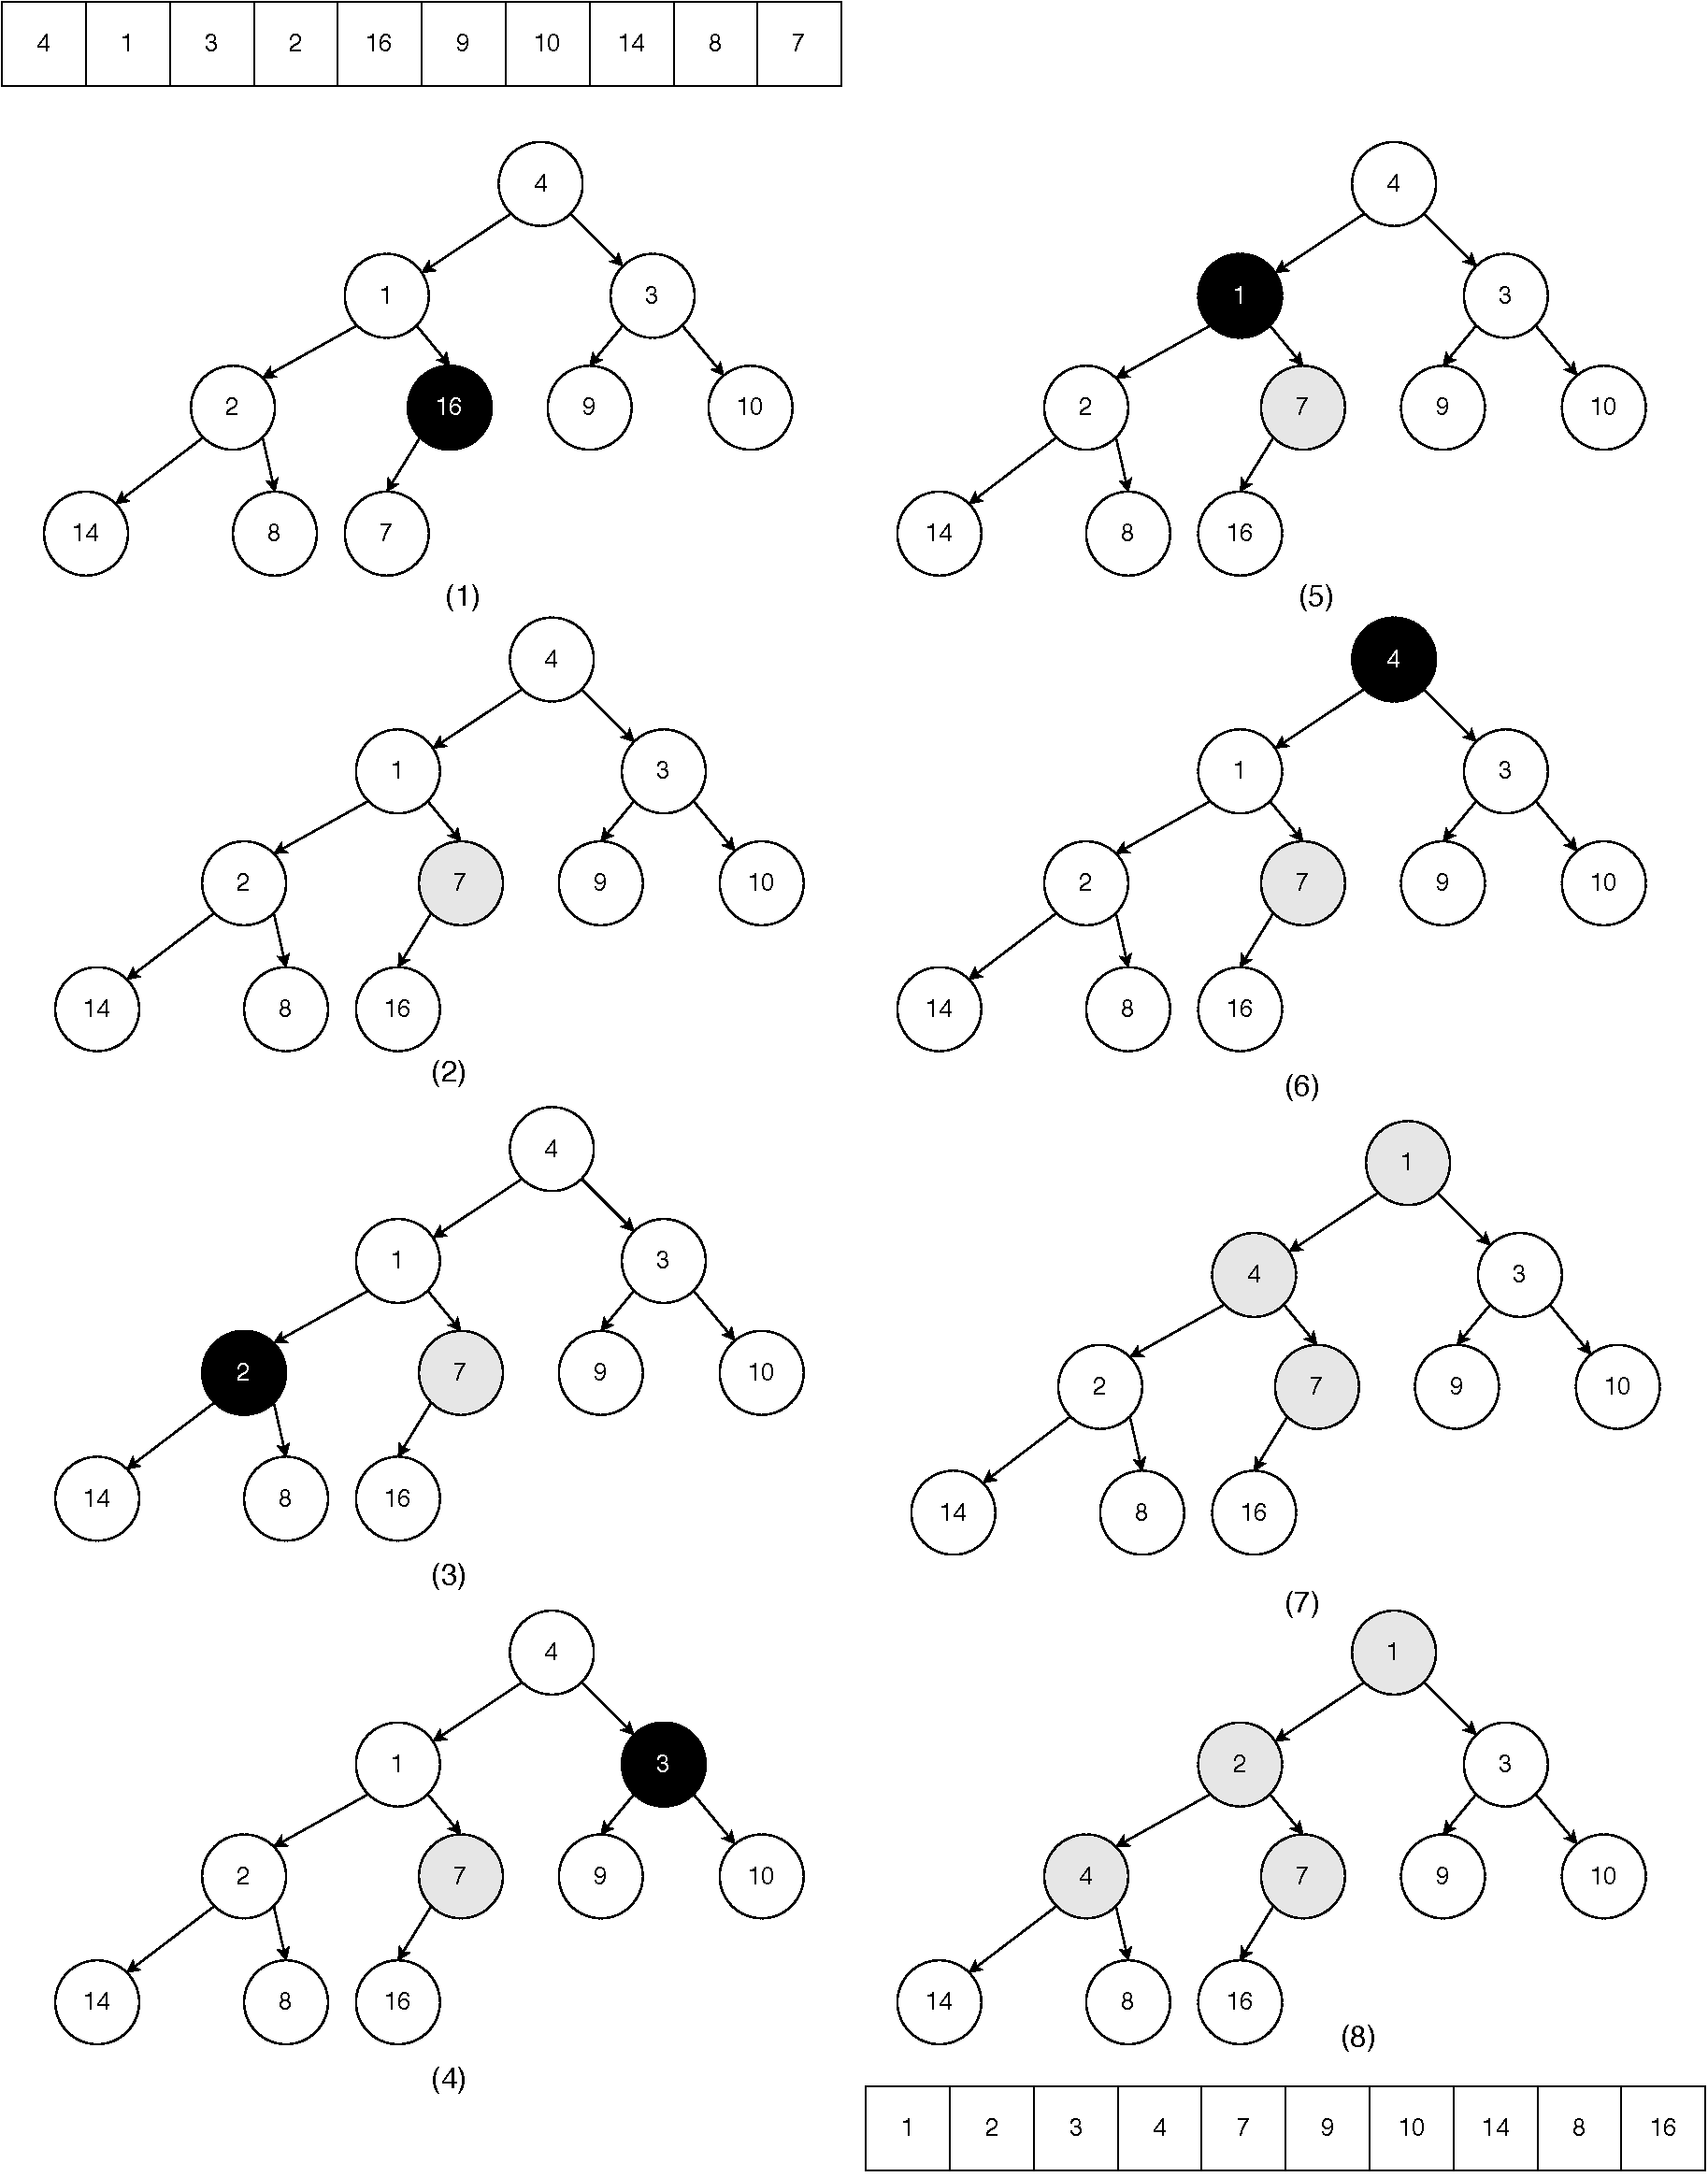
\includegraphics[scale=0.4]{img/build-heap}
  \caption{构造堆。(1)检查16,它大于子节点7;(2)交换16 $\leftrightarrow$ 7;(3)检查2,它比14,8都小;(4)检查3,它比9和10都小;(5)检查1,它比2和7都小;(6)检查4,1比4和3更小;(7)交换4 $\leftrightarrow$ 1;(8)交换4 $\leftrightarrow$ 2,结束。}
  \label{fig:build-heap-3}
\end{figure}

\subsection{堆的基本操作}

堆的基本操作包括获取顶部,弹出顶部,寻找最小(或最大)的前$k$个元素,减小小顶堆中某一元素(或增大大顶堆中某一元素),以及插入新元素。在用二叉树实现的堆中,根节点保存了顶部元素,它对应数组的第一个值:

\index{二叉堆!获取顶部元素}
\begin{algorithmic}[1]
\Function{Top}{$A$}
  \State \Return $A[1]$
\EndFunction
\end{algorithmic}

\subsubsection{弹出堆顶}
\index{二叉堆!弹出} \index{二叉堆!pop}

弹出堆顶后,数组剩余元素顺次向前移动,有可能不再满足堆性质,需要执行\textproc{Heapify}检查并调整:

\begin{algorithmic}[1]
\Function{Pop-Slow}{$A$}
  \State $x \gets$ \Call{Top}{$A$}
  \State \Call{Remove}{$A$, 1} \Comment{线性时间移动剩余元素}
  \If{$A$ is not empty}
    \State \Call{Heapify}{$A$, 1}
  \EndIf
  \State \Return $x$
\EndFunction
\end{algorithmic}

从长度为$n$的数组中删除第一个元素需要线性时间$O(n)$将剩余元素顺次向前移动一位。为了避免移动,我们可以将待移除的头部交换到数组的末尾,然后将数组的长度减一:

\begin{algorithmic}[1]
\Function{Pop}{$A$}
  \State $x \gets A [1], n \gets |A|$
  \State \textproc{Exchange} $A[1] \leftrightarrow A[n]$
  \State \Call{Remove}{$A, n$}
  \If{$A$ is not empty}
    \State \Call{Heapify}{$A$, 1}
  \EndIf
  \State \Return $x$
\EndFunction
\end{algorithmic}

从数组的末尾删除元素仅需常数时间,这样弹出操作的时间复杂度就取决于\textproc{Heapify},为$O(\lg n)$。

\subsubsection{Top-$k$}
\index{二叉堆!top-k}

连续使用pop,可以找出一组元素中的前$k$个最小(或最大):

\begin{algorithmic}[1]
\Function{Top-k}{$A, k$}
  \State $R \gets [\ ]$
  \State \Call{Build-Heap}{$A$}
  \Loop \ \textproc{Min}(k, |$A$|) times \Comment{$k$超出长度则截断}
    \State \textproc{Append}($R$, \Call{Pop}{$A$})
  \EndLoop
  \State \Return $R$
\EndFunction
\end{algorithmic}

\subsubsection{提升优先级}
\index{二叉堆!提升优先级}

堆的一个应用是实现带有优先级的任务调度,称为“优先级队列”。将若干带有优先级的任务放入堆中,每次从堆顶取出优先级最高的任务执行。为了尽早执行堆中的某个任务,可以提升它的优先级。对于小顶堆,这意味着减小某个元素的值,如图\ref{fig:decrease-key-2}所示。

\begin{figure}[htbp]
  \centering
  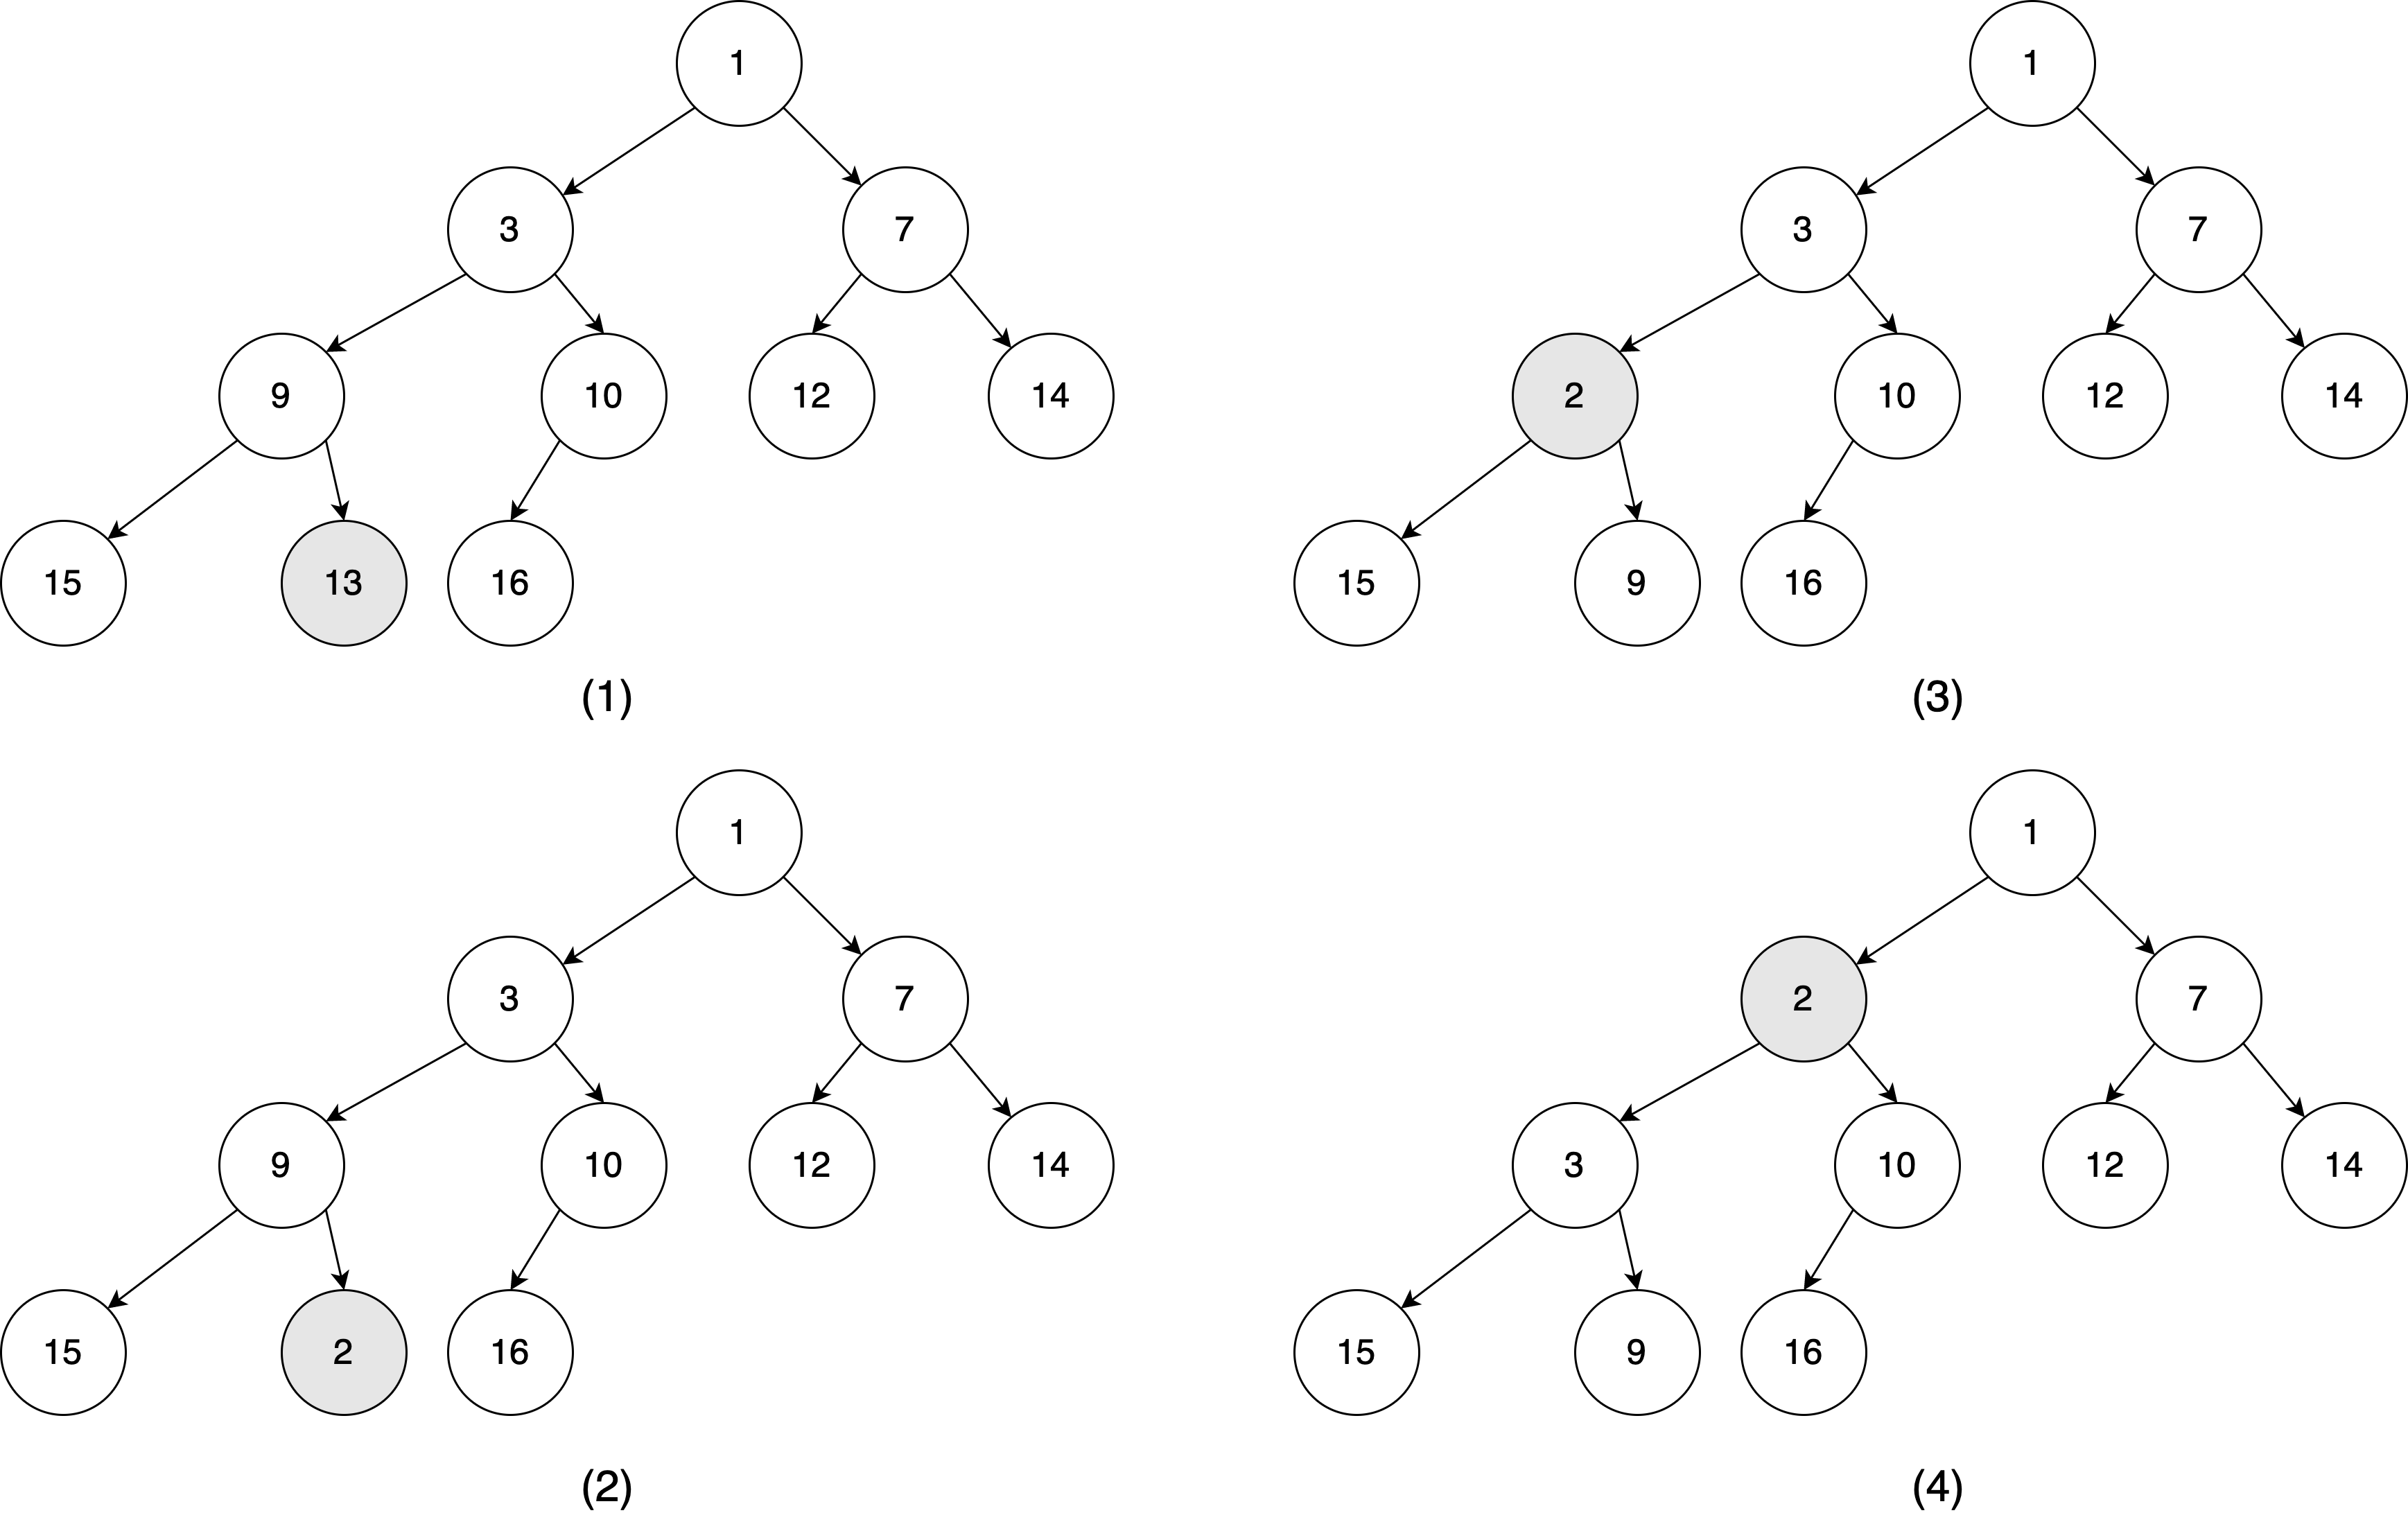
\includegraphics[scale=0.4]{img/decrease-key}
  \caption{将13减小为2。2先与9交换,然后再与3交换。}
  \label{fig:decrease-key-2}
\end{figure}

减小小顶堆中的某个元素时,可能会破坏堆性质。对于数组表示的二叉堆,令修改的元素索引为$i$,下面的算法自底向上恢复堆性质,其时间复杂度为$O(\lg n)$。

\begin{algorithmic}[1]
\Function{Heap-Fix}{$A, i$}
  \While{$i>1$ and $A[i] < A[$ \Call{Parent}{$i$} $]$}
    \State \textproc{Exchange} $A[i] \leftrightarrow A[$ \Call{Parent}{$i$} $]$
    \State $i \gets$  \Call{Parent}{$i$}
  \EndWhile
\EndFunction
\end{algorithmic}

\subsubsection{插入}
\index{二叉堆!插入(push)}

可以利用\textproc{Heap-Fix}来实现插入\cite{CLRS}。以小顶堆为例,先向数组末尾添加新元素$k$,再使用\textproc{Heap-Fix}调整:

\begin{algorithmic}[1]
\Function{Heap-Push}{$A, k$}
  \State \Call{Append}{$A, k$}
  \State \Call{Heap-Fix}{$A, |A|$}
\EndFunction
\end{algorithmic}

\subsection{堆排序}
\label{heap-sort} \index{堆排序}

可以利用堆实现排序。以小顶堆为例,从待排序元素构建一个堆,不断从堆顶获取最小元素,就获得了升序结果。若待排序的元素有$n$个,构建堆的时间复杂度是$O(n)$。由于弹出操作的复杂度为$O(\lg n)$,并且共执行了$n$次。因此总体时间复杂度为$O(n \lg n)$。由于我们使用了另外一个列表存放排序结果,因此空间复杂度为$O(n)$。

\begin{algorithmic}[1]
\Function{Heap-Sort}{$A$}
  \State $R \gets [\ ]$
  \State \Call{Build-Heap}{$A$}
  \While{$A \neq [\ ]$}
    \State \textproc{Append}($R$, \Call{Heap-Pop}{$A$})
  \EndWhile
  \State \Return $R$
\EndFunction
\end{algorithmic}

Robert. W. Floyd给出了另一种实现。思路是构建一个大顶堆。接下来,将堆顶的最大元素和数组末尾的元素交换,这样最大元素就存储到了排序后的正确位置。而原来在末尾的元素变成了新的堆顶。我们将堆的大小减一,然后执行\textproc{Heapify}恢复堆的性质。重复这一过程,直到堆中仅剩下一个元素。这一算法省去了额外的空间。

\begin{algorithmic}[1]
\Function{Heap-Sort}{$A$}
  \State \Call{Build-Max-Heap}{$A$}
  \State $n \gets |A|$
  \While{$n > 1$}
    \State \textproc{Exchange} $A[1] \leftrightarrow A[n]$
    \State $n \gets n - 1$
    \State \Call{Heapify}{$A[1...n], 1$}
  \EndWhile
\EndFunction
\end{algorithmic}


\begin{Exercise}
\begin{itemize}
\item 考虑另外一种实现原地堆排序的方法:第一步先从待排序数组构建一个最小堆$A$,此时,第一个元素$a_1$已经在正确的位置了。接下来,将剩余的元素$\{a_2, a_3, ..., a_n\}$当成一个新的堆,并从$a_2$开始执行\textproc{Heapify}。重复这一从左向右的步骤完成排序。下面的C语言代码实现了这一想法。这一方法正确么?如果正确,请给出证明,如果错误,请指出原因。
\lstset{language=C}
\begin{lstlisting}
void heap_sort(Key* a, int n) {
    build_heap(a, n, less);
    while(--n)
        heapify(++a, 0, n, less);
}
\end{lstlisting}

\item 基于同样的道理,我们可以通过自左向右执行$k$遍\textproc{Heapify}来实现原地修改的top-$k$算法么?如下面的C语言例子代码所示:
\lstset{language=C}
\begin{lstlisting}
int tops(int k, Key* a, int n, Less lt) {
    build_heap(a, n, lt);
    for (k = MIN(k, n) - 1; k; --k)
        heapify(++a, 0, --n, lt);
    return k;
}
\end{lstlisting}
\end{itemize}
\end{Exercise}

% ================================================================
%                 Explicit binary heap
% ================================================================
\section{左偏堆和skew堆―显式的二叉堆}
\label{ebheap}

人们很自然会问:如果不使用数组,有没有可能使用普通的二叉树来实现堆?

如果使用显式的二叉树作为堆的底层数据结构,我们必须解决一些问题。第一个问题是关于\textproc{Heap-Pop}和\textproc{Delete-Min}操作的。考虑图\ref{fig:lvr}所示的二叉树$(L, k, R)$,其中$L$、$k$、$R$分别表示左子树、key和右子树。

\begin{figure}[htbp]
    \centering
    \includegraphics[scale=0.8]{img/lvr}
    \caption{二叉树,所有子节点中的元素都大于$k$} \label{fig:lvr}
\end{figure}

如果$k$是一个最小堆的顶部元素,所有左右子树中的元素都大于$k$。$k$被弹出后,只剩下左右子树。我们需要把它们合并为一棵新树。由于合并后必须保持堆的性质,新的根节点必须仍保存剩余元素中的最小元素。

因为左右子树也都是符合堆性质的二叉树,我们可以立即给出两个特殊情况下的结果:

\[
merge(H_1, H_2) = \left \{
  \begin{array}
  {r@{\quad:\quad}l}
  H_2 & H_1 = \phi \\
  H_1 & H_2 = \phi \\
  ? & otherwise
  \end{array}
\right.
\]

其中$\phi$表示空堆。如果左右子树都不为空,因为它们都满足堆的性质,因此各自的根节点都保存了最小的元素。我们可以比较两棵树的根,选择较小的一个作为堆合并后的根。

举例来说,令$L = (A, x, B)$、$R = (A', y, B')$,其中$A$、$A'$、$B$、$B'$都是子树,如果$x < y$,$x$就将是新的根。我们或者可以保留$A$,然后递归地将$B$和$R$合并;或者保留$B$,然后递归地合并$A$和$R$。新的堆可以为下面之一:

\begin{itemize}
\item $(merge(A, R), x, B)$
\item $(A, x, merge(B, R))$
\end{itemize}

两个都是正确的结果,为了简单,我们可以总选择右侧的子树进行合并。左偏堆({\em Leftist} heap)就是基于这一思想实现的。

% ================================================================
%                 Definition
% ================================================================
\subsection{定义}
\index{左偏堆}

使用左偏树实现的堆称为左偏堆。左偏树最早由C. A. Crane于1972年引入\cite{wiki-leftist-tree}。

\subsubsection{Rank(S-值)}
\index{左偏堆!rank}
\index{左偏堆!S-值}

左偏树中每个节点都定义了一个Rank值(或称$S$值)。Rank被定义为到达最近的外部节点的距离。其中外部节点指空节点NIL,例如叶子节点的子节点就是外部节点。

如图\ref{fig:rank}所示,NIL的Rank被定义为0。考虑根节点4,最近的叶子节点为8,所以根节点的Rank为2。因为节点6和节点8都是叶子节点,所以它们的Rank为1。虽然节点5则左子树不为空,但是它的右子树是空节点,因此Rank值,也就是到达NIL的最短距离仍然为1。

\begin{figure}[htbp]
   \begin{center}
     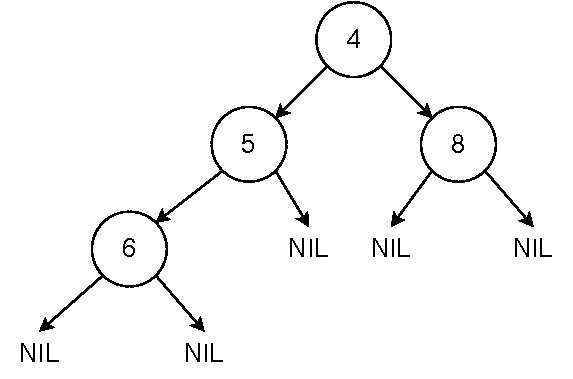
\includegraphics[scale=0.5]{img/rank}
     \caption{$rank(4) = 2$、$rank(6) = rank(8) = rank(5) = 1$} \label{fig:rank}
   \end{center}
\end{figure}

\subsubsection{左偏性质}

使用Rank,我们可以定义合并时的策略:

\begin{itemize}
\item 总是合并右侧子树。记新的右侧子树的Rank值为$r_r$;
\item 比较左右子树的Rank值,记左子树的Rank值为$r_l$,如果$r_l < r_r$,就交换左右子树。
\end{itemize}

我们称上面的合并策略为“左偏性质”。概括来说,在一棵左偏树中,到某个外部节点的最短距离总是在右侧。

左偏树总是趋向不平衡,但是它可以维护一条重要的性质,如下面的定理所述:

\begin{theorem}
若一棵左偏树$T$包含$n$个内部节点,从根节点到达最右侧的外部节点的路径上最多含有$\lfloor \log (n+1) \rfloor$个节点。
\end{theorem}

我们这里省略了此定理的证明,读者可以参考\cite{brono-book},\cite{TAOCP-bheap}来了解证明的过程。根据此定理,沿着这一路径进行操作的算法,都可以保证$O(\lg n)$的复杂度。

我们可以在二叉树定义的基础上增加一个Rank值来定义左偏树。记非空的左偏树为$(r, k, L, R)$。下面的Haskell例子程序定义了左偏树。

\lstset{language=Haskell}
\begin{lstlisting}[style=Haskell]
data LHeap a = E -- 空
             | Node Int a (LHeap a) (LHeap a) -- Rank、元素、左、右子树
\end{lstlisting}

我们定义空树的Rank为0,否则,我们通过读取新增加的变量$r$来获得Rank值。下面的$rank(H)$函数可以获取任一情况下的值。

\be
rank(H) = \left \{
  \begin{array}
  {r@{\quad:\quad}l}
  0 & H = \phi \\
  r & H = (r, k, L, R)
  \end{array}
\right.
\ee

对应的Haskell例子程序如下:

\lstset{language=Haskell}
\begin{lstlisting}[style=Haskell]
rank E = 0
rank (Node r _ _ _) = r
\end{lstlisting}

方便起见,我们以后将$rank(H)$简记为$r_H$。

% ================================================================
%                 Merge
% ================================================================
\subsection{合并}
\index{左偏堆!合并}

为了实现合并操作,我们需要显定义一个算法用以比较左右子树的Rank值,并适当地进行子树的交换。

\be
mk(k, A, B) = \left \{
  \begin{array}
  {r@{\quad:\quad}l}
  (r_A + 1, k, B, A) & r_A < r_B \\
  (r_B + 1, k, A, B) & otherwise
  \end{array}
\right.
\ee

这一函数接受三个参数,一个key和两棵子树$A$、$B$。如果$A$的Rank较小,算法就用$B$作为左子树,$A$作为右子树来构建一棵较大的树。然后它将$A$的Rank加一作为这棵新树的Rank值,即新树的Rank值为$r_A + 1$;否则,如果$B$的Rank较小,就用A作为左子树,$B$作为右子树。新树的Rank值为$r_B + 1$。

由于构造新树的时候,我们在顶部增加了一个新的key。所以Rank的值会增长1。

给定两个左偏堆$H_1$和$H_2$,记它们的key和左右子树分别为:$k_1, L_1, R_1$和$k_2, L_2, R_2$。下面的$merge(H_1, H_2)$函数定义了合并算法:

\be
merge(H_1, H_2) = \left \{
  \begin{array}
  {r@{\quad:\quad}l}
  H_2 & H_1 = \phi \\
  H_1 & H_2 = \phi \\
  mk(k_1, L_1, merge(R_1, H_2)) & k_1 < k_2 \\
  mk(k_2, L_2, merge(H_1, R_2)) & otherwise
  \end{array}
\right.
\ee

函数$merge$总是在右子树上进行递归调用,因此左偏的性质得以保持。这样就保证了算法的复杂度为$O(\lg n)$。

下面的Haskell例子代码实现了合并算法。

\lstset{language=Haskell}
\begin{lstlisting}[style=Haskell]
merge E h = h
merge h E = h
merge h1@(Node _ x l r) h2@(Node _ y l' r') =
    if x < y then makeNode x l (merge r h2)
    else makeNode y l' (merge h1 r')

makeNode x a b = if rank a < rank b then Node (rank a + 1) x b a
                 else Node (rank b + 1) x a b
\end{lstlisting}

\subsubsection{合并由数组表示的二叉堆}
\index{二叉堆!合并}

使用数组表示的二叉堆在大多数情况下速度都很快。并且很和现代计算机的高速缓存技术(cache)配合良好。但是合并操作的算法复杂度却为线性时间$O(n)$。通常的实现是将两个数组连接起来,然后在连接后的结果上重新构建堆\cite{NIST}。

\begin{algorithmic}[1]
\Function{Merge-Heap}{$A, B$}
  \State $C \gets$ \Call{Concat}{$A, B$}
  \State \Call{Build-Heap}{$C$}
\EndFunction
\end{algorithmic}

% ================================================================
%                 Basic heap operations
% ================================================================
\subsection{基本堆操作}

使用此前定义的$merge$算法,我们可以实现很多基本的堆操作。

\subsubsection{获取顶部元素和弹出操作}
\index{左偏堆!top}
\index{左偏堆!pop}
\index{左偏堆!弹出}

由于最小的元素总是存储于根节点,我们可以在常数时间$O(1)$内获取到堆的顶部元素。下式从非空的堆$H = (r, k, L, R)$中获取顶部元素。我们忽略了树为空时的错误处理。

\be
top(H) = k
\ee

为了实现弹出操作,我们首先将顶部元素删除,然后将左右子树合并为一个新的堆。

\be
pop(H) = merge(L, R)
\ee

由于弹出算法的实现直接调用了$merge$函数,因此左偏树弹出操作的复杂度也是$O(\lg n)$。

\subsubsection{插入}
\index{左偏树!插入}

我们可以从待插入的元素构建一棵只有一个叶子节点的树,然后将它和已有的左偏树合并到一起。

\be
insert(H, k) = merge(H, (1, k, \phi, \phi))
\ee

显然,由于直接调用$merge$函数,这一算法的复杂度也是$O(\lg n)$。

使用插入操作,我们可以很容易地将一个列表中的元素依次插入到左偏堆中。下面的构造算法使用了folding。

\be
build(L) = fold(insert, \phi, L)
\ee

图\ref{fig:leftist-tree}给出另一个构造左偏树的例子。

\begin{figure}[htbp]
   \begin{center}
   	  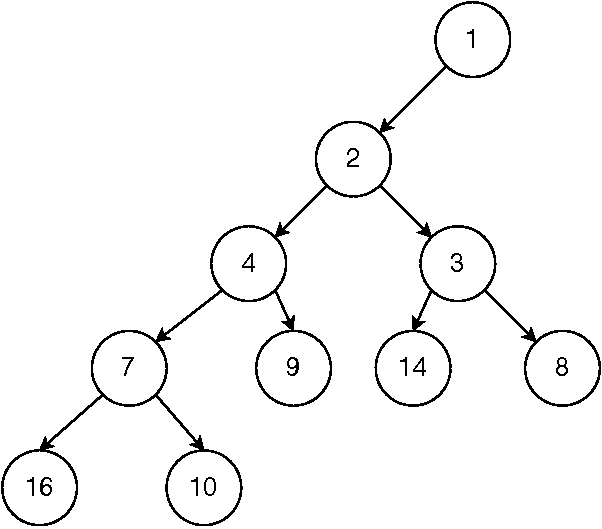
\includegraphics[scale=0.5]{img/leftist-tree}
    \caption{从列表$\{9, 4, 16, 7, 10, 2, 14, 3, 8, 1\}$构造左偏树}
    \label{fig:leftist-tree}
   \end{center}
\end{figure}

下面的Haskell例子程序实现了上面的各个左偏树操作。

\lstset{language=Haskell}
\begin{lstlisting}[style=Haskell]
insert h x = merge (Node 1 x E E) h

findMin (Node _ x _ _) = x

deleteMin (Node _ _ l r) = merge l r

fromList = foldl insert E
\end{lstlisting}

% ================================================================
%                 Heap sort
% ================================================================
\subsection{使用左偏堆实现堆排序}
\index{左偏树!堆排序}

使用堆的基本操作,我们可以给出堆排序的实现。给定一个序列,我们首先将它转换成一个左偏堆,然后不断从堆中取得最小元素。

\be
sort(L) = heapSort(build(L))
\ee

\be
heapSort(H) = \left \{
  \begin{array}
  {r@{\quad:\quad}l}
  \phi & H = \phi \\
  \{top(H)\} \cup heapSort(pop(H)) & otherwise
  \end{array}
\right.
\ee

因为弹出操作的复杂度是对数时间的,并且被调用了$n$次,因此排序的总体复杂度为$O(n \lg n)$。下面的Haskell例子程序实现了左偏树的堆排序。

\lstset{language=Haskell}
\begin{lstlisting}[style=Haskell]
heapSort = hsort . fromList where
    hsort E = []
    hsort h = (findMin h):(hsort $ deleteMin h)
\end{lstlisting} %$



% ================================================================
%                 Skew Heap
% ================================================================

\subsection{Skew堆}
\label{skew-heap}
\index{Skew堆}

左偏堆在某些情况下会产生很不平衡的结构。图\ref{fig:unbalanced-leftist-tree}给出了一个例子,依次将序列$\{16, 14, 10, 8, 7, 9, 3, 2, 4, 1\}$中的元素插入到左偏堆。

\begin{figure}[htbp]
   \begin{center}
   	  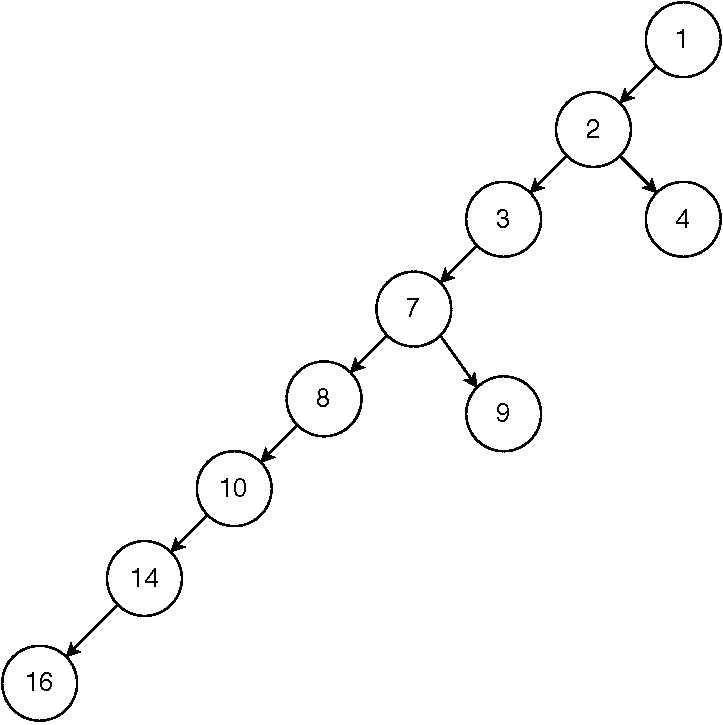
\includegraphics[scale=0.3]{img/unbalanced-leftist-tree}
    \caption{从序列$\{16, 14, 10, 8, 7, 9, 3, 2, 4, 1\}$构造的左偏堆很不平衡}
    \label{fig:unbalanced-leftist-tree}
   \end{center}
\end{figure}

Skew堆(或称\underline{自调整堆})既简化了左偏堆的实现,又提高了平衡性\cite{wiki-skew-heap}、\cite{self-adjusting-heaps}。

在构造左偏堆的时候,如果左侧的Rank值小于右侧的,我们就交换左右子树。但是这一“比较―交换”的策略在merge时不能很好处理某一分支为叶子节点的情况。这是因为,不管这棵树有多大,它的Rank值总为1。一种“简单粗暴”的解决方式是,每次合并,我们都交换左右子树。这就是Skew堆的原理。

\subsubsection{Skew堆的定义}

Skew堆是由skew树实现的堆。Skew树是一种特殊的二叉树。最小的元素保存在根节点,每棵子树也都是一棵skew树。

Skew树无需保存Rank值(或$S$值)。我们可以直接复用二叉树的定义。树或者为空,或者记为前序形式$(k, L, R)$。下面的Haskell例子代码定义了skew树。

\lstset{language=Haskell}
\begin{lstlisting}[style=Haskell]
data SHeap a = E -- 空
             | Node a (SHeap a) (SHeap a) -- 元素、左、右
\end{lstlisting}

\subsubsection{合并}
\index{Skew堆!合并}
\index{Skew堆!插入}
\index{Skew堆!top}
\index{Skew堆!pop}
\index{Skew堆!弹出}

合并算法被大幅度简化:当合并两棵非空skew树时,我们比较根节点,选择较小的作为新的根。然后把含有较大元素的树合并到某一子树上。最后再把左右子树交换。记两棵非空子树为:$H_1 = (k_1, L_1, R_1)$和$H_2 =(k_2, L_2, R_2)$。若$k_1 < k_2$,选择$k_1$作为新的根。我们既可以将$H_2$和$L_1$合并,也可以将$H_2$和$R_1$合并。不失一般性,我们合并到$R_1$上。然后交换左右子树,最后的结果为$(k_1, merge(R_1, H_2), L_1)$。考虑边界情况,最终的算法定义如下:

\be
merge(H_1, H_2) = \left \{
  \begin{array}
  {r@{\quad:\quad}l}
  H_1 & H_2 = \phi \\
  H_2 & H_1 = \phi \\
  (k_1, merge(R_1, H_2), L_1) & k_1 < k_2 \\
  (k_2, merge(H_1, R_2), L_2) & otherwise
  \end{array}
\right.
\ee

其他的操作,包括插入,获取顶部元素和弹出都和左偏树一样通过调用merge来实现。唯一的不同是我们不再需要Rank了。

下面的Haskell例子程序实现了skew堆。

\lstset{language=Haskell}
\begin{lstlisting}element, left, right
merge E h = h
merge h E = h
merge h1@(Node x l r) h2@(Node y l' r') =
    if x < y then Node x (merge r h2) l
    else Node y (merge h1 r') l'

insert h x = merge (Node x E E) h

findMin (Node x _ _) = x

deleteMin (Node _ l r) = merge l r
\end{lstlisting}

即使我们用skew堆处理已序序列,结果仍然是一棵较平衡的二叉树,如图\ref{fig:skew-tree}所示。

\begin{figure}[htbp]
   \begin{center}
   	  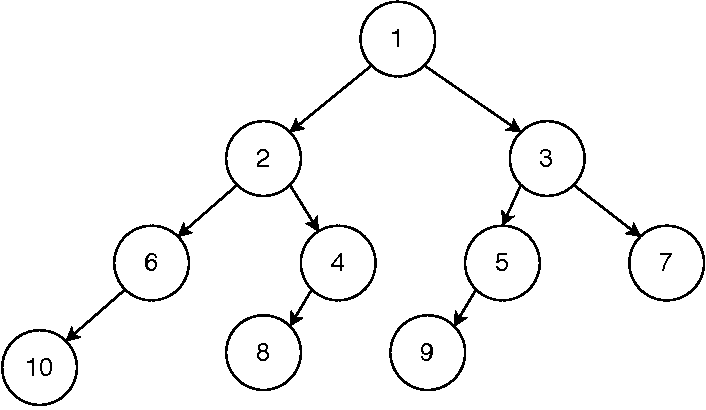
\includegraphics[scale=0.5]{img/skew-tree}
    \caption{用已序序列$\{1, 2, ..., 10\}$构造的skew树仍然比较平衡}
    \label{fig:skew-tree}
   \end{center}
\end{figure}


% ================================================================
%                 Splay Heap
% ================================================================

\section{伸展堆}
\label{splayheap}
\index{伸展堆}

左偏堆和skew堆说明,使用二叉树完全可以实现堆这种数据结构。而且skew堆还给出了一种解决树平衡的方法。本节介绍的伸展堆给出了另外一种改善平衡性的方法。

左偏堆和skew堆使用的树都不是二叉搜索树(BST)。如果我们将底层的数据结构换成二叉搜索树,最小(或最大)元素就不再保存于根节点。我们需要$O(\lg n)$时间来获取最小(或最大)元素。

如果二叉搜索树不平衡,性能会大幅下降。最坏情况下,大部分操作都退化为$O(n)$。虽然我们可以用红黑树来实现二叉堆,但这太复杂了。伸展树提供了一种轻量级的实现,它的结果可以动态趋向平衡。


% ================================================================
%                 Definition
% ================================================================
\subsection{定义}

伸展树采用类似于缓存(cache)的策略,它不断将当前正在访问的节点向top旋转,这样再次访问的时候就可以更快。我们将这样的操作称为“伸展(splay)”。对于不平衡的二叉搜索树,经过若干次伸展操作后,树会变得越来越平衡。大多数伸展树操作的均摊(amortized)性能都是$O(\lg n)$的。Daniel Dominic Sleator和Robert Endre Tarjan在1985年最早引入了伸展树\cite{wiki-splay-tree}\cite{self-adjusting-trees}。

\subsubsection{伸展操作}
\index{伸展堆!splaying}

有两种方法可以实现伸展操作。第一种需要处理较多的情况,但可以很容易地使用模式匹配(pattern matching)来实现;第二种具备统一的形式,但是实现较为复杂。

记当前正在访问的节点为$X$,它的父节点为$P$,如果存在祖父节点,则记为$G$。伸展操作分为三各步骤,每个步骤有两个对称的情况,为了节省篇幅,我们只给出每步中的一种情况。

\begin{itemize}
\item \underline{Zig-zig}步骤,如图\ref{fig:zig-zig}所示,$X$和$P$都是左子树或者$X$和$P$都是右子树。我们通过两次旋转,将$X$变成根节点。

\begin{figure}[htbp]
  \centering
  \subcaptionbox{$X$和$P$都是左子树或者$X$和$P$都是右子树。}{\includegraphics[scale=0.4]{img/zig-zig-a}}
  \subcaptionbox{$X$经过两次旋转后成为了根节点。}{\includegraphics[scale=0.4]{img/zig-zig-b}}
  \caption{Zig-zig情况} \label{fig:zig-zig}
\end{figure}

\item \underline{Zig-zag}步骤,如图\ref{fig:zig-zag}所示,$X$和$P$一棵是左子树另一棵是右子树。经过旋转,$X$变成根节点,$P$和$G$变成了兄弟节点。

\begin{figure}[htbp]
  \centering
  \subcaptionbox{$X$和$P$一棵是左子树另一棵是右子树。}{\includegraphics[scale=0.4]{img/zig-zag-a}}
  \subcaptionbox{$X$成为根节点,$P$和$G$变成了兄弟节点。}{\includegraphics[scale=0.4]{img/zig-zag-b}}
  \caption{Zig-zag情况} \label{fig:zig-zag}
\end{figure}

\item \underline{Zig}步骤,如图\ref{fig:zig}所示,这种情况下,$P$是根节点,经过旋转,$X$变成了根节点。这是伸展操作的最后一步。

\begin{figure}[htbp]
  \centering
  \subcaptionbox{$P$是根节点。}{\includegraphics[scale=0.4]{img/zig-a}}
  \subcaptionbox{通过旋转将$X$变为根节点。}{\includegraphics[scale=0.4]{img/zig-b}}
  \caption{Zig情况} \label{fig:zig}
\end{figure}

\end{itemize}

虽然有6种不同的情况,但是它们可以很容易地用模式匹配来处理。记非空二叉树为$T=(L, k, R)$,当访问树中的节点$Y$时,伸展操作可以定义如下:

\be
splay(T, X) = \left \{
  \begin{array}
  {r@{\quad:\quad}l}
  (a, X, (b, P, (c, G, d))) & T = (((a, X, b), P, c), G, d), X = Y \\
  (((a, G, b), P, c), X, d) & T= (a, G, (b, P, (c, X, d))), X = Y \\
  ((a, P, b), X, (c, G, d)) & T = (a, P, (b, X, c), G, d), X = Y \\
  ((a, G, b), X, (c, P, d)) & T = (a, G, ((b, X, c), P, d)), X = Y \\
  (a, X, (b, P, c)) & T = ((a, X, b), P, c), X = Y \\
  ((a, P, b), X, c) & T = (a, P, (b, X, c)), X = Y \\
  T &  otherwise
  \end{array}
\right.
\ee

前两条子式处理“zig-zig”情况;接下来的两条子式处理“zig-zag”情况;最后两条子式处理“zig”情况。其他情况下,树都保持不变。

下面的Haskell例子程序实现了伸展操作。

\lstset{language=Haskell}
\begin{lstlisting}[style=Haskell]
data STree a = E -- 空
             | Node (STree a) a (STree a) -- left, key, right

-- zig-zig
splay t@(Node (Node (Node a x b) p c) g d) y =
    if x == y then Node a x (Node b p (Node c g d)) else t
splay t@(Node a g (Node b p (Node c x d))) y =
    if x == y then Node (Node (Node a g b) p c) x d else t
-- zig-zag
splay t@(Node (Node a p (Node b x c)) g d) y =
    if x == y then Node (Node a p b) x (Node c g d) else t
splay t@(Node a g (Node (Node b x c) p d)) y =
    if x == y then Node (Node a g b) x (Node c p d) else t
-- zig
splay t@(Node (Node a x b) p c) y = if x == y then Node a x (Node b p c) else t
splay t@(Node a p (Node b x c)) y = if x == y then Node (Node a p b) x c else t
-- 否则
splay t _ = t
\end{lstlisting}

每次插入新key时,我们就执行伸展操作来调整树的平衡性。如果树为空,结果为一个叶子节点;否则我们比较待插入的key和根节点,如果待插入的key较小,就将其递归插入左子树,然后执行伸展操作;否则将key插入右子树,再执行伸展操作。

\be
insert(T, x) = \left \{
  \begin{array}
  {r@{\quad:\quad}l}
  (\phi, x, \phi) & T = \phi \\
  splay((insert(L, x), k, R), x) & T = (L, k, R), x < k \\
  splay(L, k, insert(R, x)) & otherwise
  \end{array}
  \right.
\ee

下面的Haskell程序实现了插入算法。

\lstset{language=Haskell}
\begin{lstlisting}[style=Haskell]
insert E y = Node E y E
insert (Node l x r) y
    | x > y     = splay (Node (insert l y) x r) y
    | otherwise = splay (Node l x (insert r y)) y
\end{lstlisting}

图\ref{fig:splay-result}描述了向伸展树插入逐一插入有序序列$\{1, 2, ..., 10\}$中元素的结果。如果使用普通二叉树,会退化成一条链表。而伸展树则产生比较平衡的结果。

\begin{figure}[htbp]
  \centering
  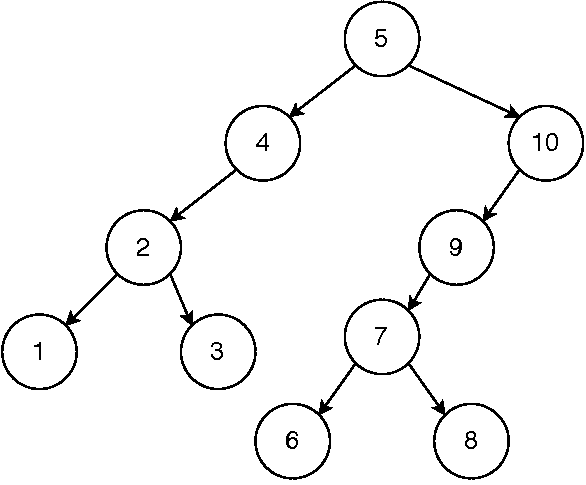
\includegraphics[scale=0.5]{img/splay-tree}
  \caption{伸展操作可以改善平衡性}
  \label{fig:splay-result}
\end{figure}

Okasaki发现了一条简单的伸展操作规则\cite{okasaki-book}:每次连续向左或者向右访问两次的时候,就旋转两个节点。

根据这一规则,我们可以这样实现伸展:当访问节点$x$的时候(插入、查找或者删除时),如果连续向左侧或者右侧前进两次,我们就将树分割成两部分:$L$和$R$,其中$L$含有所有小于$x$的节点,$R$含有其余的节点。我们可以构建一棵新树(例如插入时),将$x$作为根,$L$和$R$分别作为左右子树。分割是递归的,它会对子树也进行伸展操作。

\be
partition(T, p) = \left \{
  \begin{array}
  {r@{\quad:\quad}l}
  (\phi, \phi) & T = \phi \\
  (T, \phi) & T = (L, k, R) \land R = \phi \\
  ((L, k, L'), k', A, B) & \begin{array}{l} \\
                             T = (L, k, (L', k', R')) \\
                             k < p, k' < p \\
                             (A, B) = partition(R', p)
                           \end{array} \\
  ((L, k, A), (B, k', R')) & \begin{array}{l} \\
                               T = (L, K, (L', k', R')) \\
                               k < p \leq k' \\
                               (A, B) = partition(L', p) \\ \\
                             \end{array} \\
  (\phi, T) & T = (L, k, R) \land L = \phi \\
  (A, (L', k', (R', k, R)) & \begin{array}{l} \\
                               T = ((L', k', R'), k, R) \\
                               p \leq k, p \leq k' \\
                               (A, B) = partition(L', p)
                             \end{array} \\
  ((L', k', A), (B, k, R)) & \begin{array}{l} \\
                               T = ((L', k', R'), k, R) \\
                               k' \leq p \leq k \\
                               (A, B) = partition(R', p)
                             \end{array}
  \end{array}
  \right.
\ee

函数$partition(T, p)$接受一棵树$T$和一个基准值(pivot)$p$为参数。第一条子式处理边界条件。对空树进行分割的结果为一对空的左右子树。否则,记树为$(L, k, R)$,我们需要比较基准值$p$和根节点的值$k$。如果$k < p$,分为两种子情况。一种是$R$为空的简单情况,根据二叉搜索树的性质,所有的元素都小于$p$,因此结果为$(T, \phi)$。

否则,$R = (L', k', R')$,我们需要递归地用基准值分割$R'$,将$R'$中所有小于$p$的元素放入树$A$,其余元素放入树$B$。结果为一对树,其中一棵为$((L, k, L'), k', A)$,另一棵为$B$。

如果右子树的key不小于基准值,我们递归地用基准值分割$L'$得到结果$(A, B)$。最终的结果为一对树,一棵是$(L, k, A)$,另一棵是$(B, k', R')$。当$p \leq k$时,情况是对称的,由最后的三条子式处理。

下面的Haskell例子程序实现了分割算法。

\begin{lstlisting}[style=Haskell]
partition E _ = (E, E)
partition t@(Node l x r) y
    | x < y =
        case r of
          E -> (t, E)
          Node l' x' r' ->
              if x' < y then
                  let (small, big) = partition r' y in
                  (Node (Node l x l') x' small, big)
              else
                  let (small, big) = partition l' y in
                  (Node l x small, Node big x' r')
    | otherwise =
        case l of
          E -> (E, t)
          Node l' x' r' ->
              if y < x' then
                  let (small, big) = partition l' y in
                  (small, Node l' x' (Node r' x r))
              else
                  let (small, big) = partition r' y in
                  (Node l' x' small, Node big x r)
\end{lstlisting}

% ================================================================
%                 Basic heap operations
% ================================================================
\index{伸展堆!插入}
我们可以用$partition$实现插入算法。当向一个伸展堆$T$插入一个新元素$k$时,我们先将堆分割为两棵子树$L$和$R$。其中$L$含有所有小于$k$的节点,而$R$含有剩余的部分。然后我们构建一棵新树,使用$k$作为根,$L$和$R$作为子树。

\be
insert(T, k) = (L, k, R), (L, R) = partition(T, k)
\ee

对应的Haskell例子程序如下:

\lstset{language=Haskell}
\begin{lstlisting}[style=Haskell]
insert t x = Node small x big where (small, big) = partition t x
\end{lstlisting}

\subsubsection{获取和弹出顶部元素}
\index{伸展堆!top}
\index{伸展堆!pop}
\index{伸展堆!弹出}

由于伸展树本质上是二叉搜索树,最小的元素存储于最左侧的节点中。我们需要不断向左遍历以获取顶部元素。记非空的树为$T=(L, k, R)$,$top(T)$函数可以定义如下:

\be
top(T) = \left \{
  \begin{array}
  {r@{\quad:\quad}l}
  k & L = \phi \\
  top(L) & otherwise
  \end{array}
  \right.
\ee

这实际上就是二叉搜索树的$min(T)$算法。

对于弹出操作,算法需要将最小元素删除。每当连续向左访问两次,就执行一次伸展操作。

\be
pop(T) = \left \{
  \begin{array}
  {r@{\quad:\quad}l}
  R & T = (\phi, k, R) \\
  (R', k, R) & T = ((\phi, k', R'), k, R) \\
  (pop(L'), k', (R', k, R)) & T = ((L', k', R'), k, R)
  \end{array}
  \right.
\ee

注意这里的第三条子式实际上执行了伸展操作,它并没有显式地调用$partition$函数,而是直接使用了二叉搜索树的性质。

因为伸展树是平衡的,top和pop操作的性能都是$O(\lg n)$。

下面的Haskell例子程序实现了top和pop操作。

\lstset{language=Haskell}
\begin{lstlisting}[style=Haskell]
findMin (Node E x _) = x
findMin (Node l x _) = findMin l

deleteMin (Node E x r) = r
deleteMin (Node (Node E x' r') x r) = Node r' x r
deleteMin (Node (Node l' x' r') x r) = Node (deleteMin l') x' (Node r' x r)
\end{lstlisting}

\subsubsection{合并}
\index{伸展堆!合并}

合并是堆的一个重要操作,它被广泛用于图算法。通过使用$partition$函数,我们可以实现一个$O(\lg n)$时间的合并算法。

当合并两棵伸展树时,如果它们都不为空,我们可以将第一棵树的根节点作为新的根,然后将其作为基准值分割第二棵树。此后,我们递归地将第一棵树的子树合并。算法定义如下:

\be
merge(T_1, T_2) = \left \{
  \begin{array}
  {r@{\quad:\quad}l}
  T_2 & T_1 = \phi \\
  (merge(L, A), k, merge(R, B)) & T_1 = (L, k, R), (A, B) = partition(T_2, k)
  \end{array}
  \right.
\ee

如果第一个堆为空,结果显然为第二个堆。否则,记第一个堆为$(L, k, R)$,我们使用$k$作为基准值分割$T_2$得到结果$(A, B)$,其中$A$包含$T_2$中所有小于$k$的节点,而$B$包含其余节点。我们接下来递归地将$A$和$L$合并为新的左子树,将$B$和$R$合并为右子树。

这一定义可以翻译为下面的Haskell例子程序。

\lstset{language=Haskell}
\begin{lstlisting}[style=Haskell]
merge E t = t
merge (Node l x r) t = Node (merge l l') x (merge r r')
    where (l', r') = partition t x
\end{lstlisting}

% ================================================================
%                 Heap sort
% ================================================================
\subsection{堆排序}

由于伸展堆的内部实现对于通用堆的接口完全透明,我们可以完全复用此前的堆排序定义。也就是说堆排序的算法也是通用的,它不依赖于底层的数据结构。

% ================================================================
%                 Short summary
% ================================================================
\section{小结}

本章中,我们介绍了通用的二叉堆概念。只要保证堆的性质,我们可以使用任何形式的二叉树来实现堆。

这样的定义并不仅限于使用基于数组的二叉堆,它也包含使用其他二叉树形式的堆如左偏堆、skew堆和伸展堆。基于数组的二叉堆易于用命令式的方式实现。它将一棵完全二叉树映射为数组的随机访问,我们很难找到和它直接对应的纯函数式实现。

但是,我们可以通过使用显式的二叉树来实现纯函数式的二叉堆。大部分的操作在最坏情况下也可以达到$O(\lg n)$的性能。有些操作的分摊性能甚至可以达到$O(1)$。Okasaki在\cite{okasaki-book}中给出了这些数据结构的详细分析。

我们仅在本章中给出了左偏堆、skew堆和伸展堆的纯函数式实现。它们也都支持命令式实现。

人们很自然希望能将二叉树扩展到$k$叉树,这样就会得到其他重要的数据结构如二项式(Binomial)堆、斐波那契(Fibonacci)堆和配对(pairing)堆。我们将在后面的章节加以介绍。

% ================================================================
%                 Exercise
% ================================================================
\begin{Exercise}
\begin{itemize}
\item 用命令式的方式实现左偏堆、skew堆和伸展堆。
\end{itemize}
\end{Exercise}

\section{附录:例子程序}

在数组表示的完全二叉树中,利用位运算访问父节点和子树,索引从0开始:

\begin{lstlisting}[language = Bourbaki]
Int parent(Int i) = ((i + 1) >> 1) - 1

Int left(Int i) = (i << 1) + 1

Int right(Int i) = (i + 1) << 1
\end{lstlisting}

堆调整的例子实现,元素比较运算抽象为参数:

\begin{lstlisting}[language = Bourbaki]
void heapify([K] a, Int i, Less<K> lt) {
    Int l, r, m
    Int n = length(a)
    loop {
        m = i
        l = left(i)
        r = right(i)
        if l < n and lt(a[l], a[i]) then m = l
        if r < n and lt(a[r], a[m]) then m = r
        if m != i {
            swap(a, i, m);
            i = m
        } else {
            break
        }
    }
}
\end{lstlisting}

从数组构造堆:

\begin{lstlisting}[language = Bourbaki]
void buildHeap([K] a, Less<K> lt) {
    Int n = length(a)
    for Int i = (n-1) / 2 downto 0 {
        heapify(a, i, lt)
    }
}
\end{lstlisting}

弹出堆顶:

\begin{lstlisting}[language = Bourbaki]
K pop([K] a, Less<K> lt) {
    var n = length(a)
    t = a[n]
    swap(a, 0, n - 1)
    remove(a, n - 1)
    if a != [] then heapify(a, 0, lt)
    return t
}
\end{lstlisting}

寻找top-$k$:

\begin{lstlisting}[language = Bourbaki]
[K] topk([K] a, Int k, Less<K> lt) {
    buildHeap(a, lt)
    [K] r = []
    loop min(k, length(a)) {
        append(r, pop(a, lt))
    }
    return r
}
\end{lstlisting}

减小堆中某元素的值:

\begin{lstlisting}[language = Bourbaki]
void decreaseKey([K] a, Int i, K k, Less<K> lt) {
    if lt(k, a[i]) {
        a[i] = k
        heapFix(a, i, lt)
    }
}

void heapFix([K] a, Int i, Less<K> lt) {
    while i > 0 and lt(a[i], a[parent(i)]) {
        swap(a, i, parent(i))
        i = parent(i)
    }
}
\end{lstlisting}

堆插入:

\begin{lstlisting}[language = Bourbaki]
void heapPush([K] a, K k, less<K> lt) {
    append(a, k)
    heapFix(a, length(a) - 1, lt)
}
\end{lstlisting}

堆排序:

\begin{lstlisting}[language = Bourbaki]
void heapSort([K] a, less<K> lt) {
    buildHeap(a, not . lt)
    n = length(a)
    while n > 1 {
        swap(a, 0, n - 1)
        n = n - 1
        heapify(a[0 .. (n - 1)], 0, not . lt)
    }
}
\end{lstlisting}

\ifx\wholebook\relax \else
\begin{thebibliography}{99}

\bibitem{CLRS}
Thomas H. Cormen, Charles E. Leiserson, Ronald L. Rivest and Clifford Stein. ``Introduction to Algorithms, Second Edition''. The MIT Press, 2001. ISBN: 0262032937.(《算法导论》)

\bibitem{wiki-heap}
Heap (data structure), Wikipedia. \url{https://en.wikipedia.org/wiki/Heap_(data_structure)}

\bibitem{wiki-heapsort}
Heapsort, Wikipedia. \url{https://en.wikipedia.org/wiki/Heapsort}

\bibitem{okasaki-book}
Chris Okasaki. ``Purely Functional Data Structures''. Cambridge university press, (July 1, 1999), ISBN-13: 978-0521663502

\bibitem{rosetta-heapsort}
Sorting algorithms/Heapsort. Rosetta Code. \url{http://rosettacode.org/wiki/Sorting_algorithms/Heapsort}

\bibitem{wiki-leftist-tree}
Leftist Tree, Wikipedia. \url{https://en.wikipedia.org/wiki/Leftist_tree}

\bibitem{brono-book}
Bruno R. Preiss. Data Structures and Algorithms with Object-Oriented Design Patterns in Java. \url{http://www.brpreiss.com/books/opus5/index.html}

\bibitem{TAOCP-bheap}
Donald E. Knuth. ``The Art of Computer Programming. Volume 3: Sorting and Searching.''. Addison-Wesley Professional;
2nd Edition (October 15, 1998). ISBN-13: 978-0201485417. Section 5.2.3 and 6.2.3

\bibitem{wiki-skew-heap}
Skew heap, Wikipedia. \url{https://en.wikipedia.org/wiki/Skew_heap}

\bibitem{self-adjusting-heaps}
Sleator, Daniel Dominic; Jarjan, Robert Endre. ``Self-adjusting heaps'' SIAM Journal on Computing 15(1):52-69. doi:10.1137/0215004 ISSN 00975397 (1986)

\bibitem{wiki-splay-tree}
Splay tree, Wikipedia. \url{https://en.wikipedia.org/wiki/Splay_tree}

\bibitem{self-adjusting-trees}
Sleator, Daniel D.; Tarjan, Robert E. (1985), ``Self-Adjusting Binary Search Trees'', Journal of the ACM 32(3):652 - 686, doi: 10.1145/3828.3835

\bibitem{NIST}
NIST, ``binary heap''. \url{http://xw2k.nist.gov/dads//HTML/binaryheap.html}

\end{thebibliography}

\end{document}
\fi
